\chapter{Tecnologias}
%Alguma coisa aqui
\section{Arquitetura}
Para o desenvolvimento do projeto, e tendo em vista que será construída uma aplicação web de página única, utilizaremos de ferramentas que cerceiam o ecossistema de \textit{Single Page Applications}. Para isso, teremos a divisão do projeto em \textit{front-end} e \textit{back-end} de modo que eles se comuniquem via protocolo HTTP com requisições e respostas no formato JSON. Para o desenvolvimento do \textit{front-end} utilizaremos Typescript por meio da biblioteca React; o \textit{back-end} será desenvolvido utilizando Java com o \textit{framework} Spring. Um módulo de apoio no lado do servidor poderá ser possível, e para ele utilizaremos Python. 

Em relação ao deploy das aplicações, o \textit{front-end} será hospedado na plataforma Vercel, que é primariamente voltada para Javascript, proporcionando uma melhor agilidade de desenvolvimento, enquanto o \textit{back-end} será hospedado no Heroku, que é uma plataforma como serviço de fácil manuseio e que nos permitirá ter um maior foco no desenvolvimento do projeto. Através do Heroku podemos também fazer a utilização do banco de dados PostgreSQL por meio do serviço de apoio Heroku Postgres.

Ademais, se for necessário o armazenamento de objetos como arquivos ou imagens, utilizaremos a plataforma Cloudinary principalmente por sua fácil integração com a linguagem de programação Java através de bibliotecas.

%
\subsection{Diagramas de arquitetura}
Os diagramas \autoref{fig_arq_app}, \autoref{fig_arq_tec} e \autoref{fig_arq_negocio} ilustram de modo geral a arquitetura pensada para a solução proposta, utilizando das tecnologias já citadas.

\begin{figure}[htb]
	\centering
	\caption{\label{fig_arq_app}Arquitetura de Aplicação}
	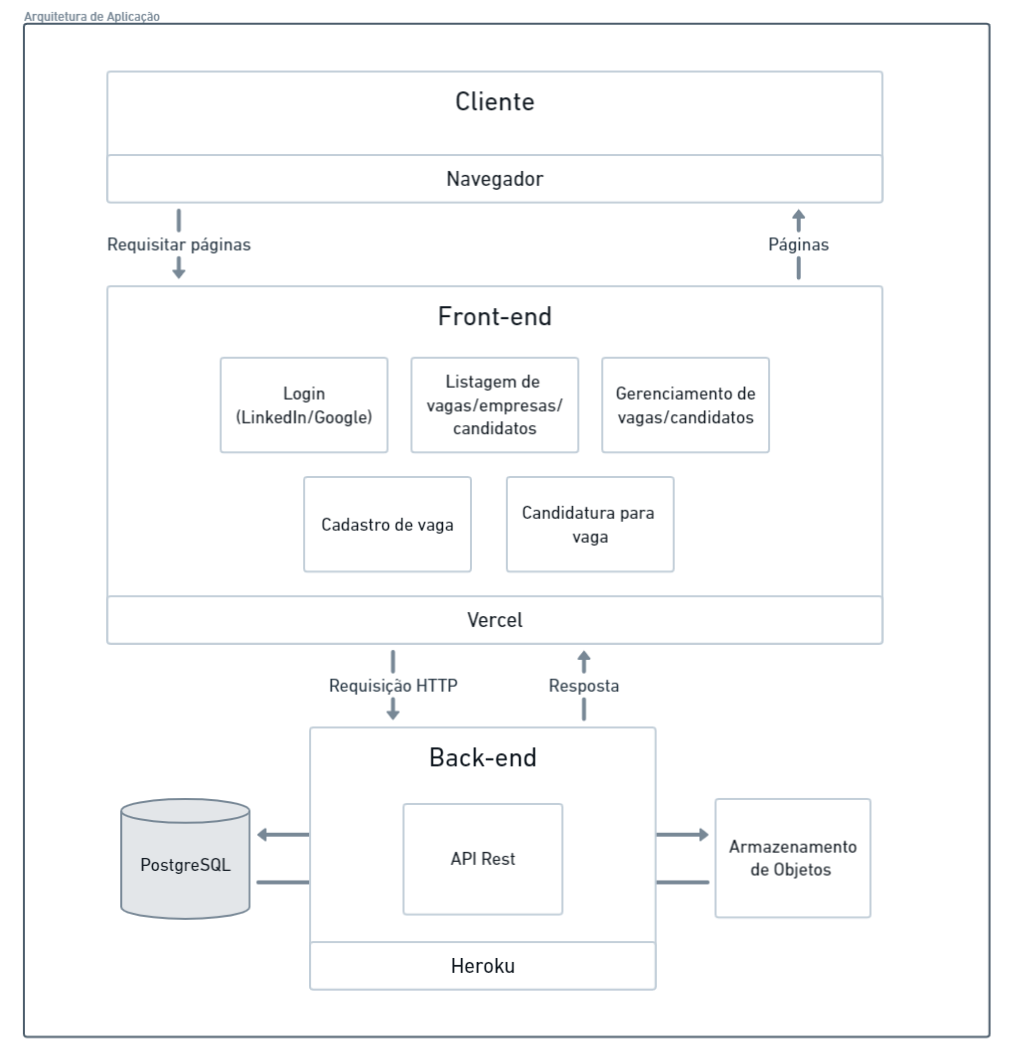
\includegraphics[width=0.95\textwidth]{../Figuras/arq-proj-arq-app.png}
	\fonte{Produzido pelos autores utilizando a ferramenta \textit{whimscal}}
\end{figure}

\begin{figure}[htb]
	\centering
	\caption{\label{fig_arq_tec}Arquitetura Tecnológica}
	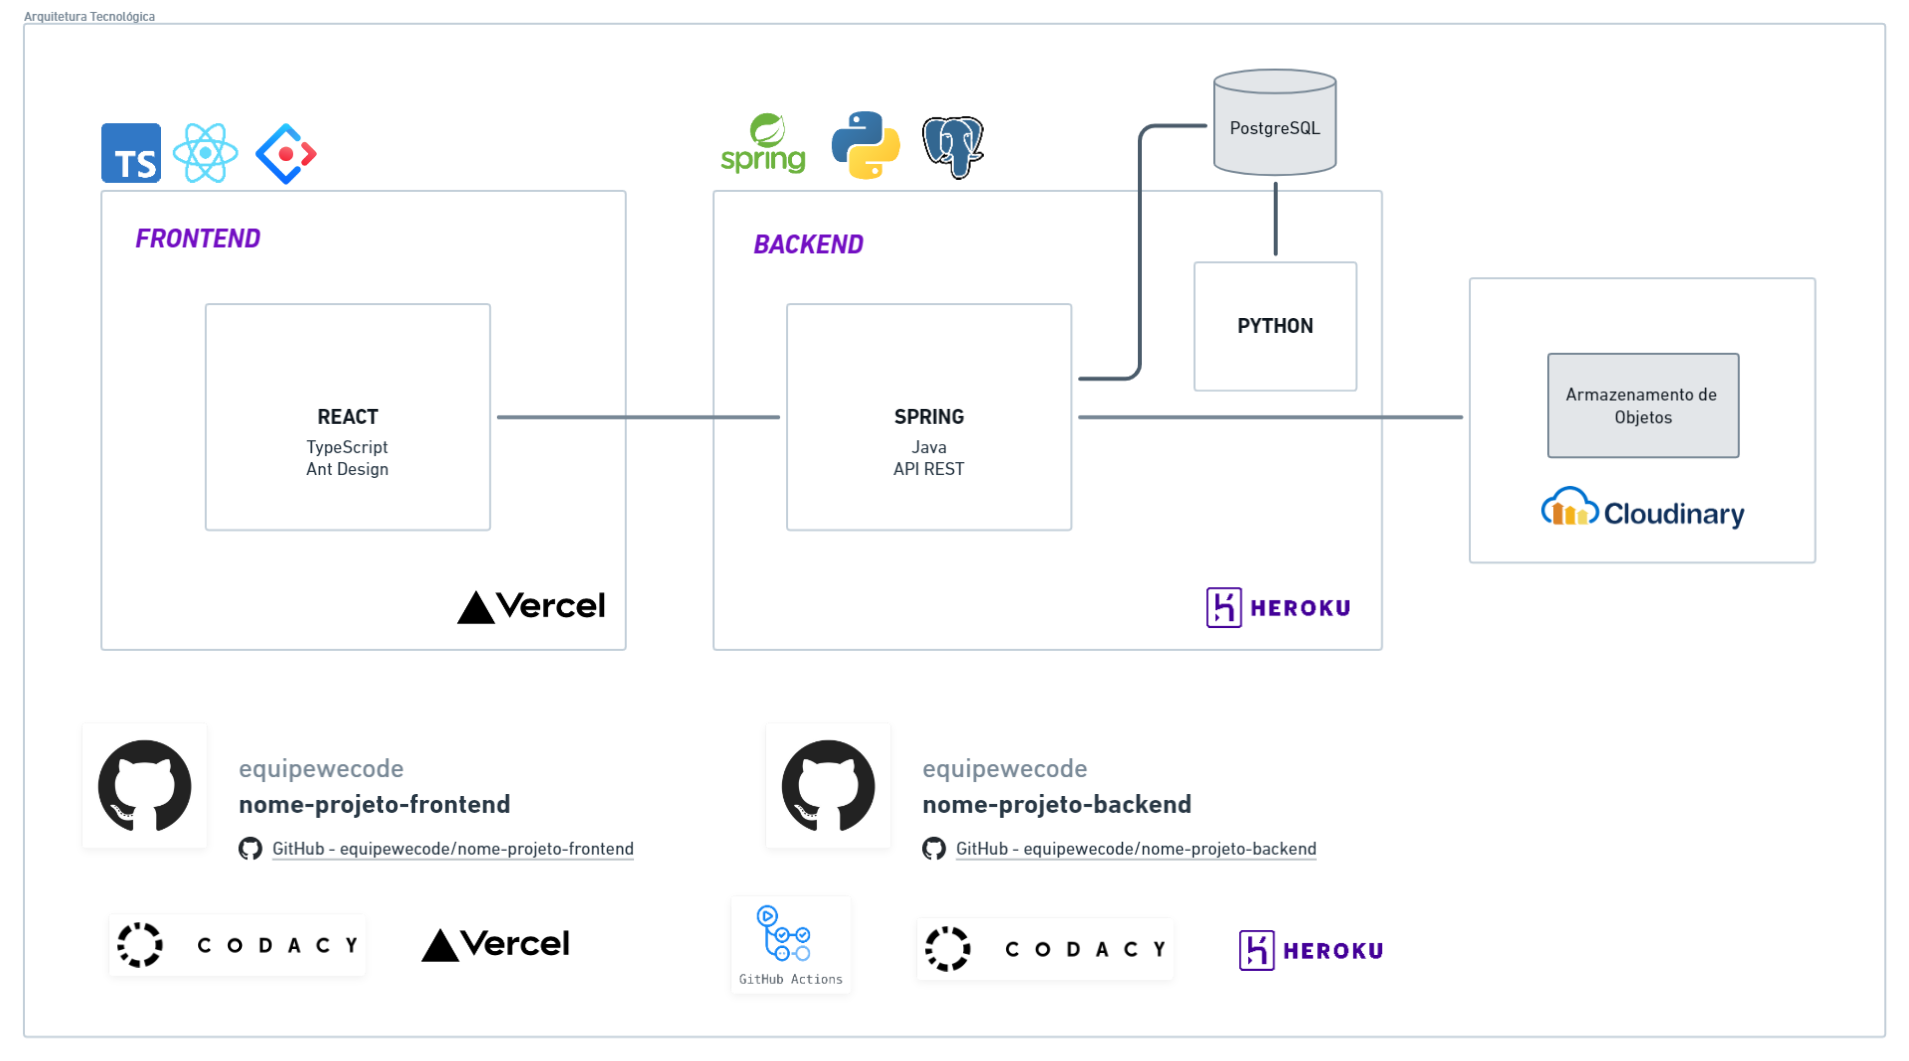
\includegraphics[width=0.95\textwidth]{../Figuras/arq-proj-arq-tec.png}
	\fonte{Produzido pelos autores utilizando a ferramenta \textit{whimscal}}
\end{figure}

\begin{figure}[htb]
	\centering
	\caption{\label{fig_arq_negocio}Arquitetura de Negócios}
	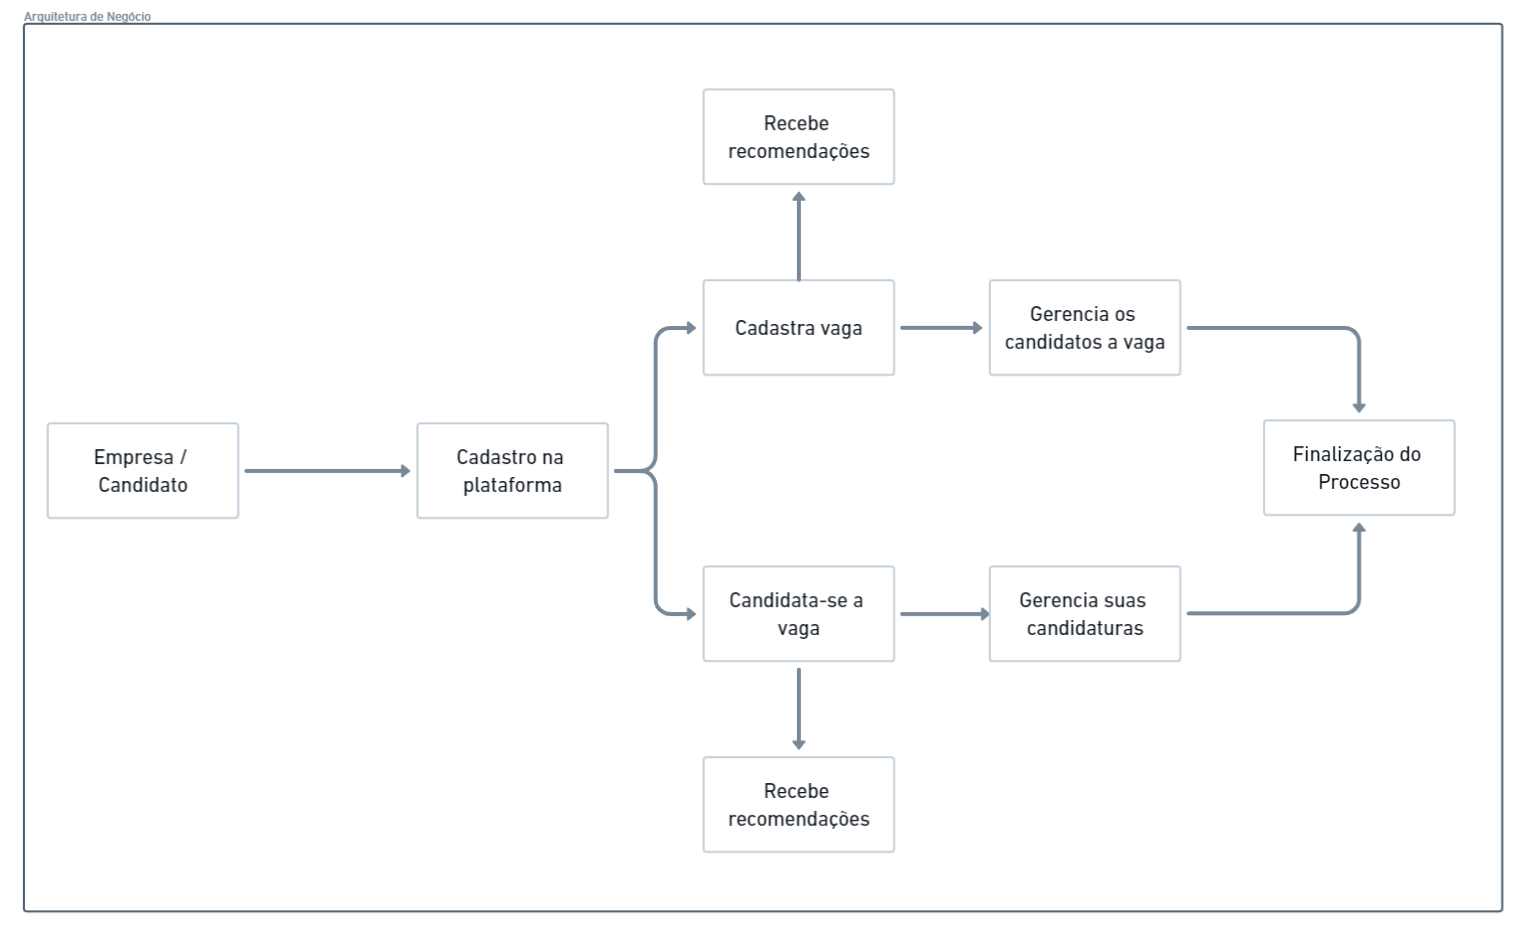
\includegraphics[width=0.95\textwidth]{../Figuras/arq-proj-arq-negocio.png}
	\fonte{Produzido pelos autores utilizando a ferramenta \textit{whimscal}}
\end{figure}

\section{Integrações}
%Login com LinkedIn e Google